%!TEX root = ../thesis.tex
%%%%%%%%%%%%%%%%%%%%%%%%%%%%%%%%%%%%%%%%%%%%%%%%%%%%%%%%%%%%%%%%%%%%%%%
%
% Introduction
%
%%%%%%%%%%%%%%%%%%%%%%%%%%%%%%%%%%%%%%%%%%%%%%%%%%%%%%%%%%%%%%%%%%%%%%%
\chapter{Introduction}
Most of the time, a software is a combination of different feature sets. In Monolithic Architecture, 
all the features of a software reside in a single a single file. If any code updates are required, 
then those updates cannot be accommodated independently. The developer must use the same code base, 
make the required code changes, and then re-deploy the updated code. So even a single change requires 
the whole code base to touched and re-deployed. 

\smallskip

The above traditional architecture comes with a major caveat, that is, beyond a point, scaling the application 
becomes disproportionately difficult, with respect to time, human resources, computer resources and storage. 
This is because of the atomic nature of resources, for example storage. A minor increase in the number of users 
and consequent requests would require a new server to be provisioned, complete with storage, compute and memory. 
This new resource would not be utilized to the fullest, until the number of users increases, thus increasing 
the request load to an optimum amount. The biggest challenge though, is when the load is not balanced or well distributed, 
and there may be a peak times requiring all the deployed resources, while during the remainder, those provisioned resources 
lie idle, which is a huge waste of resources. 

\smallskip

Another commonly use architecture, called Microservice Architecture, has gained popularity over the recent years, 
due to its ability to overcome some of the disadvantages of Monolithic Architecture. It involves splitting the application 
into multiple "microservices", or smaller, fully independent components, which can operate, scale and be maintained, 
independently of the other components. It can be said to be a mini app, complete with its own database as well. 
This comes with its own challenges of complexity, and with synchronous update of state throughout the assorted services, 
although it provides more control over the resources, and mitigates some of the scaling challenges. For example, 
if a single microservice is running out of storage, there is no need to scale the infrastructure across all the services, 
we can get away with scaling just the one we need. This raises an important conundrum though, of how much should the
application be divided, as smaller, “microservices” offer a more fine-grained control, but proportionally increases the 
complexity of the overall application. 

\smallskip

This leads us to the most recent, ever evolving and improving Serverless Architecture. A serverless architecture abstracts 
the underlying infrastructure and offers a “pay as you use” model, wherein you always only pay for the resources you need. 
If the load increases, it scales automatically, and you pay per request, and thus when the load decreases, you pay much less.

\smallskip

The main aim of this project will be to build a fully scalable architecture, using as many serverless features as possible, 
such that there is no wasting of resources, and we are billed for exactly what we use. If we see a sudden growth of users 
towards our platform, we should be able to serve them all, while if there are no visitors, our costs should be minimal. 

\textbf{Key Words}: Serverless, pay as you use, scalable architecture, dynamic load, idle resource utilization 

\subsection{Problem Statement} 

With so many providers and options for these services, it could get daunting for a new startup to decide on their technology stack and architecture, as the difference between success and failure for their venture could depend largely on how well it performs, and how economically. Thus, establishing an efficient, well defined standard for development, right from the selection of service providers to the appropriate tools to be used for the job is the need of the hour. 

\subsection{Background} 

In recent times, the technology stack used for software development has evolved from a simple, standard architecture and limited set of tools to a myriad of options, with each aspect of development and infrastructure offering choices with certain advantages and tradeoffs. These options, while good to have, have raised a conundrum, that is the abundance syndrome. Be it front-end frameworks, UI frameworks, backend frameworks, database engines or software architectures, the appropriate choice of technologies to choose is no longer an easy task.

\smallskip 

With the rise of cloud computing, large companies like Amazon, Google and Microsoft have jumped into the fray, initially offering infrastructure as a service, passing onto their customers a share into the economy of scales they are able to leverage, thus reducing the costs of operation. To outbid their competitors, these cloud service providers started offering more managed services, with complexities abstracted behind easy to use APIs, using their experience developing software at scale to provide improved management of common requirements like, for instance, databases. Eventually, in this competitive environment, these managed services evolved into the serverless architecture we know today.  

\begin{figure}[!hb]
\centering
\caption[Cloud Computing market size]{Cloud Computing market size}%
\label{fig:cloud_computing_market_size}
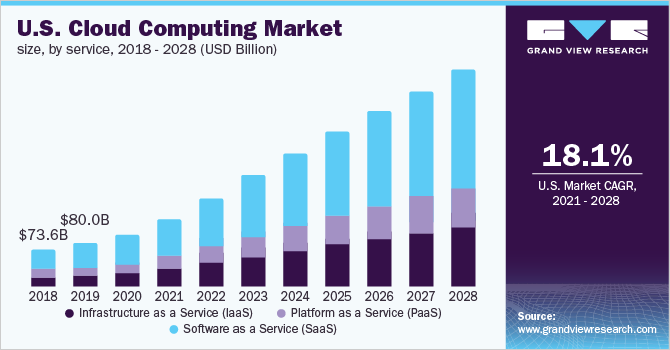
\includegraphics[width=\linewidth,height=\textheight,keepaspectratio]{img/cloud_computing_market_size}
\end{figure} 

As we can see from the above market research trends, the cloud computing market has been growing rapidly, and is expected to continue the trajectory in the long term. 

Thus, leveraging this boom and evaluating the best provider and services is of utmost importance for any company wishing to stay with the trend in the future, which looks to be heading towards managed cloud services. 

\section{Aims and Objectives} 

With a view to evaluate cloud computing offerings from various cloud service providers, this project aims to develop a cloud native vegan recipe sharing website infinitely scalable, highly efficient and economical, using the pay for what you use model. 

Furthermore, the objectives of the project are explicitly listed below:

\begin{enumerate}[label=\arabic*.]
  \item Building a full stack application, mimicking the most widespread use case for most web applications \textbf{(O1)}.
  \item Allowing users to signup and login, add recipes, delete their recipes, comment on recipes, report recipes and also browse for recipes, with extensive filtering \textbf{(O2)}.
  \item Using the most modern front-end technologies, based on React/Next and following best practices \textbf{(O3)}.
  \item Building a complete serverless backend bit by bit, using serverless offerings from popular cloud services providers like AWS (Amazon Web Services) and GCP (Google Cloud Platform), thus demonstrating a fully scalable app \textbf{(O4)}.
  \item Exploring modern data querying languages, GraphQl, in line with our main objective of reducing waste, that is querying for exactly what we need \textbf{(O5)}.
  \item Exploring tools like Amplify to create a proof-of-concept template to make provisioning all the services easy and rapid \textbf{(O6)}.
\end{enumerate}

\section{Project Scope} 

The project scope encompasses the analysis, design, implementation and evaluation of a cloud-native, 
web-based system (as stated in the objectives) that is able to mimic the most widespread web applications, 
like that of a blog \textbf{(O1)}. It would allow users to register, login, add recipes, search and filter for recipes, 
edit their own recipes, as well as comment or like other recipes \textbf{(O2)}. They would also be able to report recipes 
to the admin if they feel that a recipe is not vegan, or is in violation of any rules. This project, however, 
does not allow for any orders for any of the posted recipes. It is not a food delivering or ecommerce application, 
we do not facilitate payments to any of the recipe bloggers. This project will use AWS Amplify to provision the 
resources needed for the backend, a GraphQL API and DynamoDB as the scalable serverless database \textbf{(O4, O5, O6)}.

\section{Dissertation Structure} 

For the sake of building a coherent dissertation report, this dissertation will follow a logical advancement approach, very similar to the development of the actual application. It begins with an abstract providing the gist of what we are trying to accomplish. The first chapter introduces the project to us, with details such as the aims and objectives of the project. This would immediately be followed by a literature review, where we justify our tech stack and choices with respect to cloud service providers. In the next chapter, we discuss about project management, that is the timeline of the project, schedule and software development methodology.


